\documentclass[10pt,oneside,onecolumn,letterpaper]{article}
\usepackage{graphicx}
\usepackage{xcolor}
\usepackage[hidelinks]{hyperref}
\usepackage{booktabs}
\usepackage{adjustbox}

\usepackage[top=.5in, bottom=1in, left=.5in, right=.7in]{geometry}

\usepackage{fontspec}
\setmainfont{Arial}

\begin{document}

%%
% THIS IS THE HEADER
%%
\noindent\colorbox{black}{
\begin{minipage}[c]{.99\linewidth}
  \vspace{.4cm}
  \Large{\color{white}{\textbf{\hspace{.3cm}University of Massachusetts Boston}}}
  \begin{flushright}
    \vspace{-1.2cm}
    
\includegraphics[width=3cm]{gfx/cs460.png}
  \end{flushright}
\end{minipage}
}

%%
% CONTENT STARTS HERE
%%

\vspace{.5cm} % add some space

\noindent\textbf{CS460 Fall 2019} \\
\textbf{Name:} Jared Barresi \\
\textbf{Student ID:} 00974358 \\
\textbf{Due Date:} 09/09/2019

\section*{Assignment 1: Intro}

\textbf{Describe your favorite WebGL demo.}

\vspace{.5cm} % add some space

\noindent My favorite demo is .... (\url{http://madebyevan.com/webgl-water/}). 

\vspace{.5cm}

\noindent The authors do a great job implementing a realistic looking physics simulation, that also has a simple-to-use interface for user interaction. Fluid physics/simulation has always been something that fascinates and inspires me, so this is an example of great interest.(In Addition, I was originally getting a B.S in Physics at UMB, switched only 2 semesters ago).

\vspace{.5cm} % add some space

\noindent\textbf{Images:}

\newline

\vspace{.5cm} % add some space

\noindent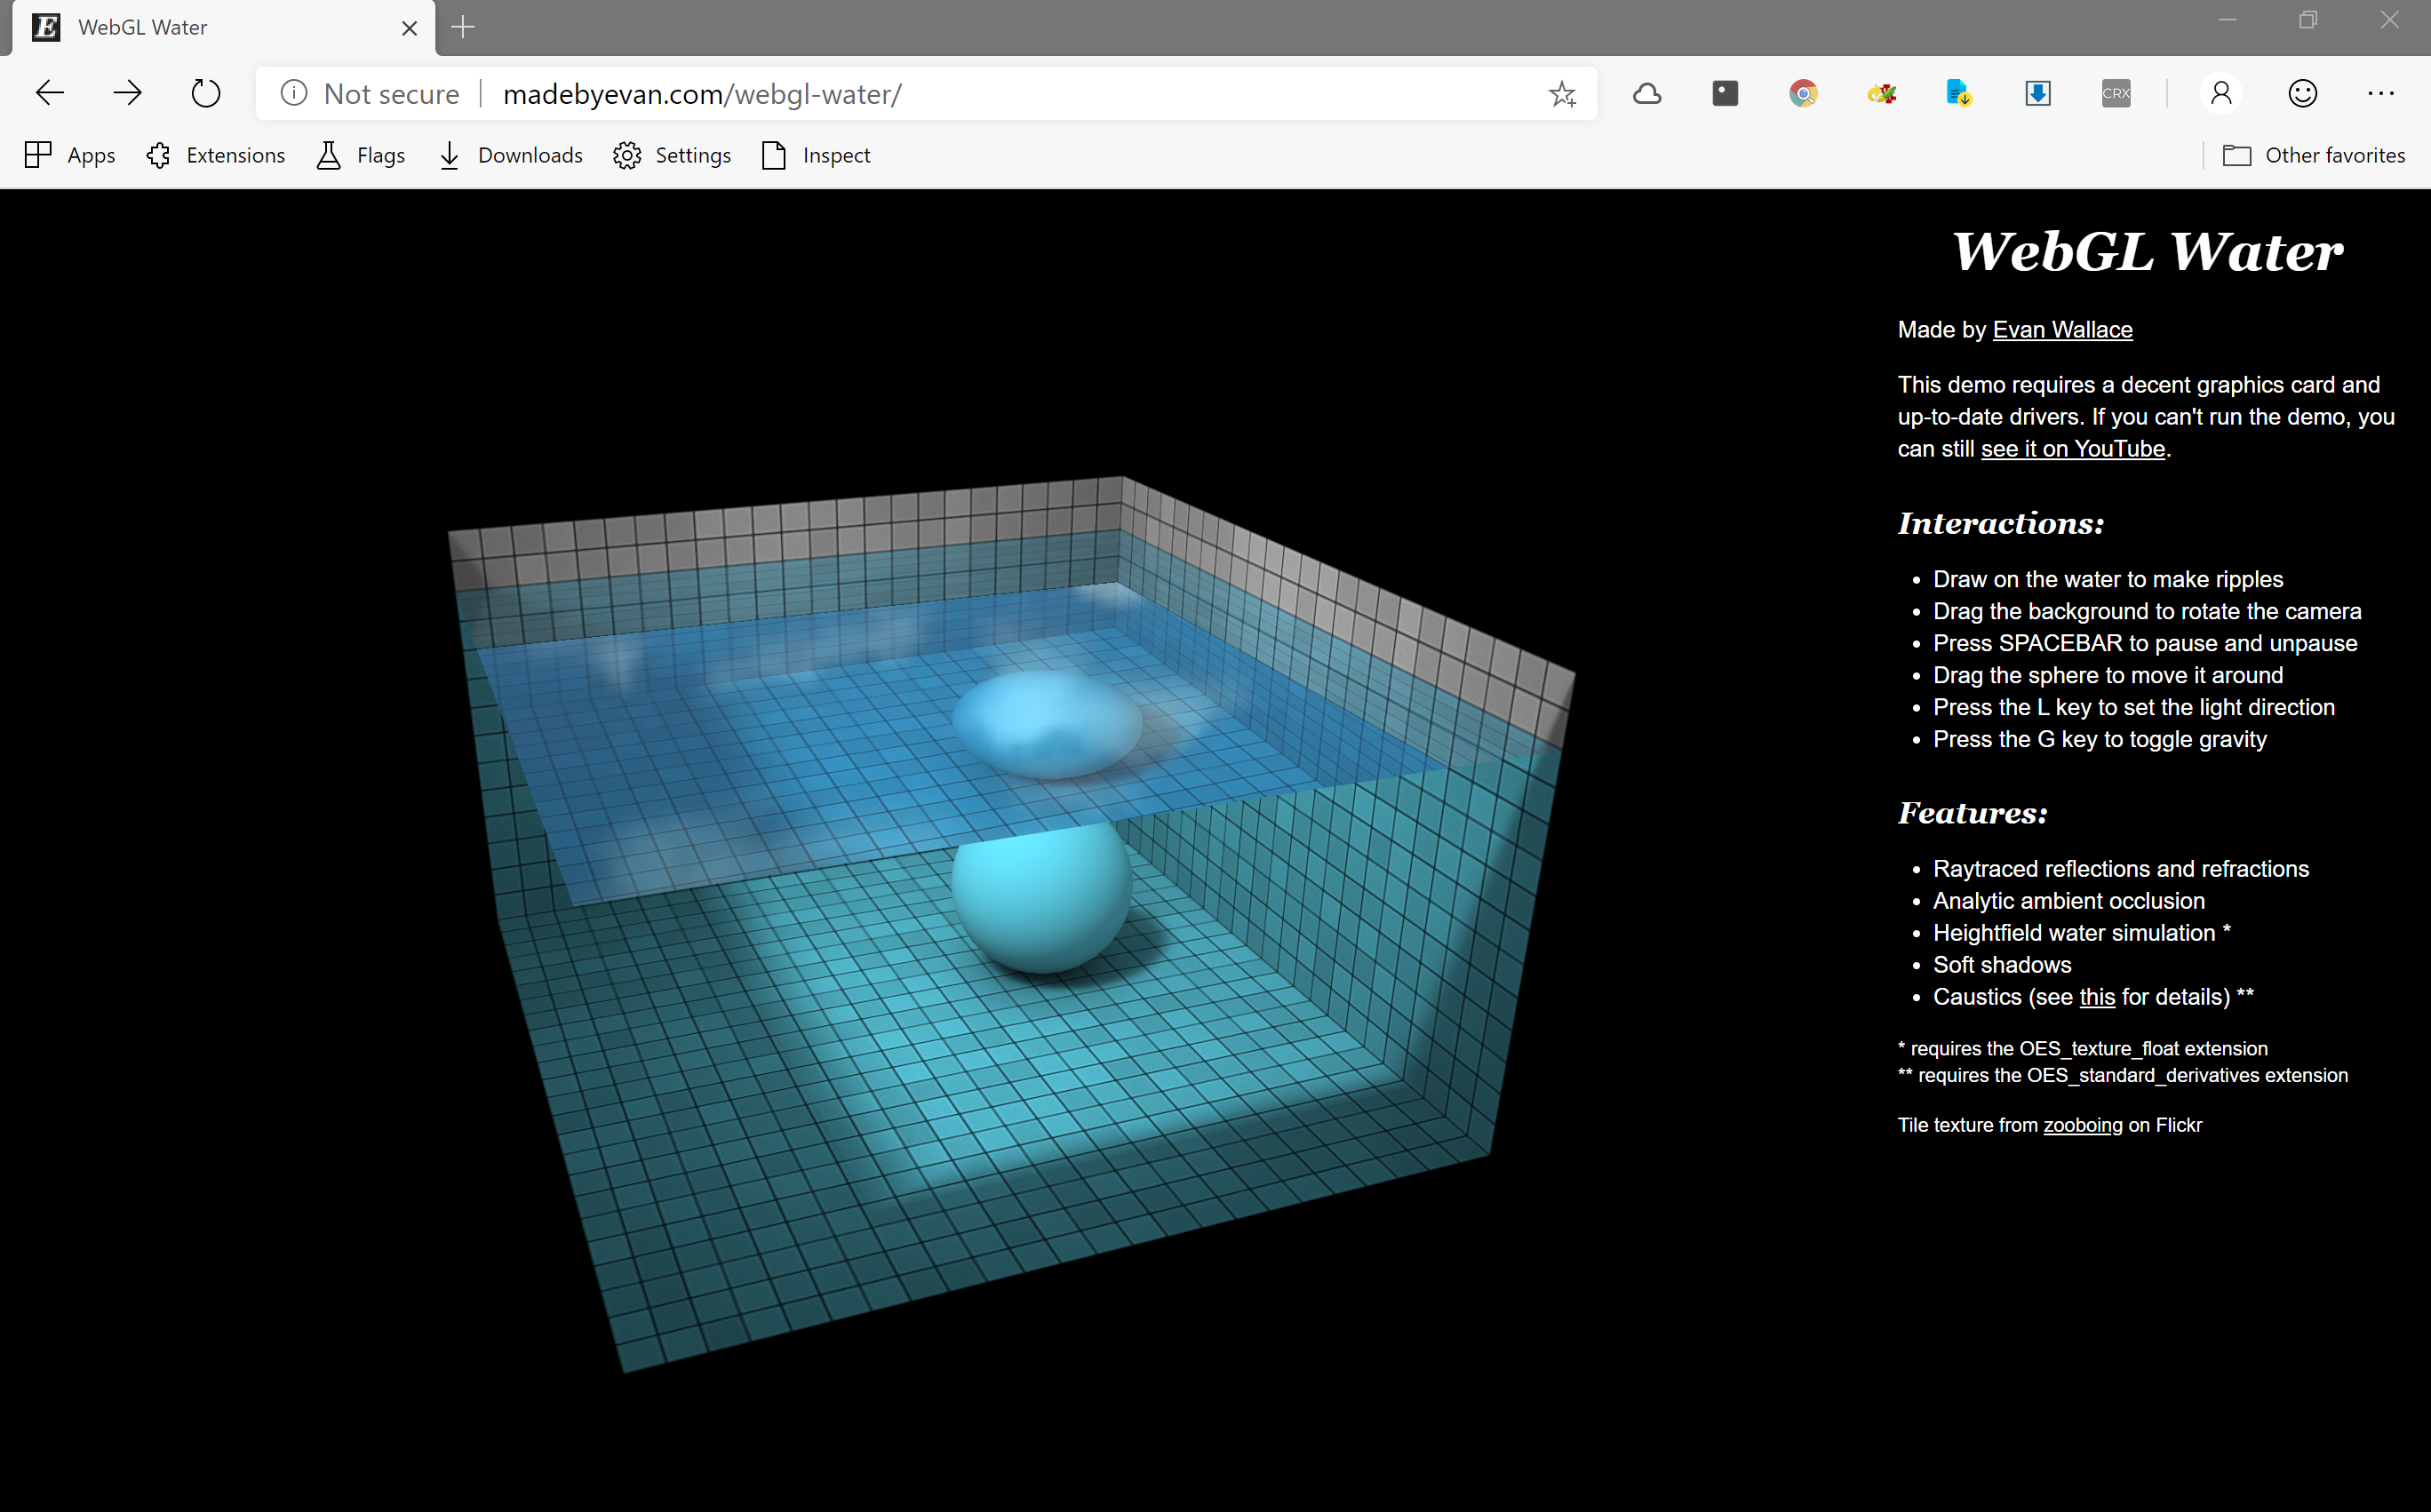
\includegraphics[width=\textwidth]{gfx/full-screenshot-madebyevan_webgl_water.png}

\vspace{.5cm}
\noindent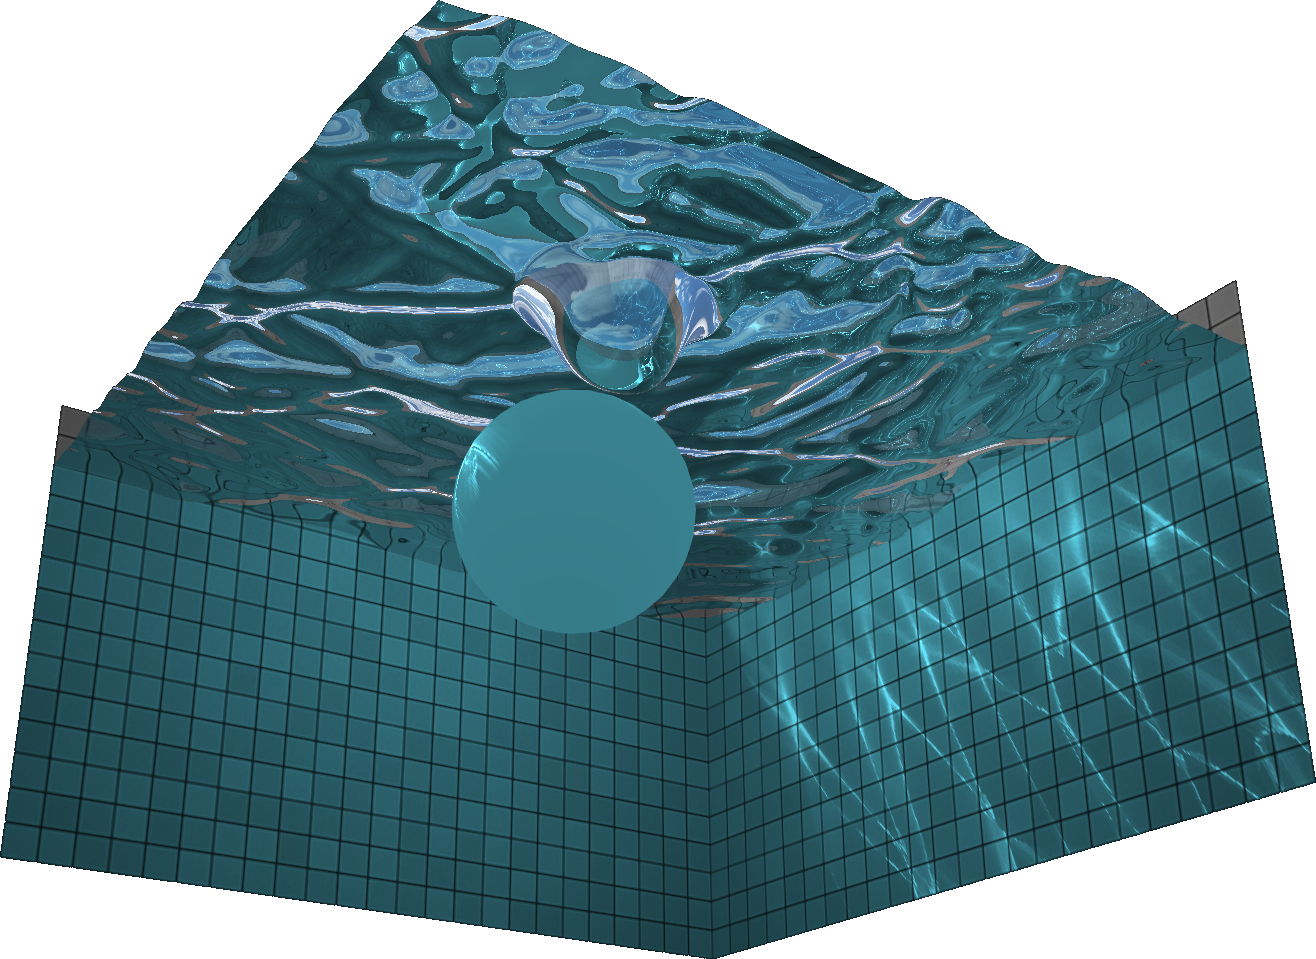
\includegraphics[width=\textwidth]{gfx/screenshot-madebyevan_webgl_water.png}

\vspace{.5cm}

\noindent\textbf{Technologies used:}

\begin{itemize}
    \item HTML/CSS/JavaScript
\end{itemize}

\noindent\textbf{Scripts:}
\begin{itemize}

    \item Three.js
    \item OES\_texture\_float\_linear-polyfill.js
    \item lightgl.js
    \item cubemap.js
    \item renderer.js
    \item water.js
    \item main.js
\end{itemize}

\vspace{.5cm}

\break

\noindent\textbf{Another favorite demo:}

\noindent Can be found at:
\noindent (\url{https://threejs.org/examples/webgl_effects_anaglyph.html}).

\vspace{.5cm}

\noindent I have done a lot of research / expressed interest in different 3D technologies, in relation to both how they work to produce 3D visuals as well as the code behind the functionality of different implementations. This is a cool demo that utilises the three.js library to make a 3D scene. I have used this in a few android apps I was working on, one of which is a series of many different demos put together into one unified test app. 

\vspace{.5cm}

\noindent\textit{It should be noted that I am refering to 3D with glasses or polarization tecniques (such as at a movie theater), for instance Anaglyph or Side By Side (SBS) 3D views.}

\vspace{.5cm}

\noindent A demo of my app can be found here (\url{https://gitlab.com/hltdev8642/AnaglyphWeb}), although it requires the Droidscript framework and app (+ an Android device) to run/test it. 

\vspace{.5cm}

\noindent\textbf{Technologies used:}
\vspace{.5cm}


\noindent\textbf{Scripts:}
\begin{itemize}
\item 3jsrc.js
\item Anaglyphs.js
\item three.min.js
\item AnaglyphWeb.js \textbf{<--[main file for runtime]}
\item three.js
\item AnaglyphDemoA.js
\item Imgur.js
\item AnaglyphEffect.js
\item google.js
\item Adapter.js
\item anaglyph.js
\item AnaglyphWebNative.js
\item Anaglyphs.js
\item DrawingPad.js
\item DualCamera.js
\item GeometryUtils.js
\item anaglyph3d.js
\item FastFourier2D.js
\item FourierCamera.js
\item anaglyph3d.packed.js
\end{itemize}

\vspace{.5cm}

\break

\noindent\textbf{Images:}

\vspace{.5cm}

\noindent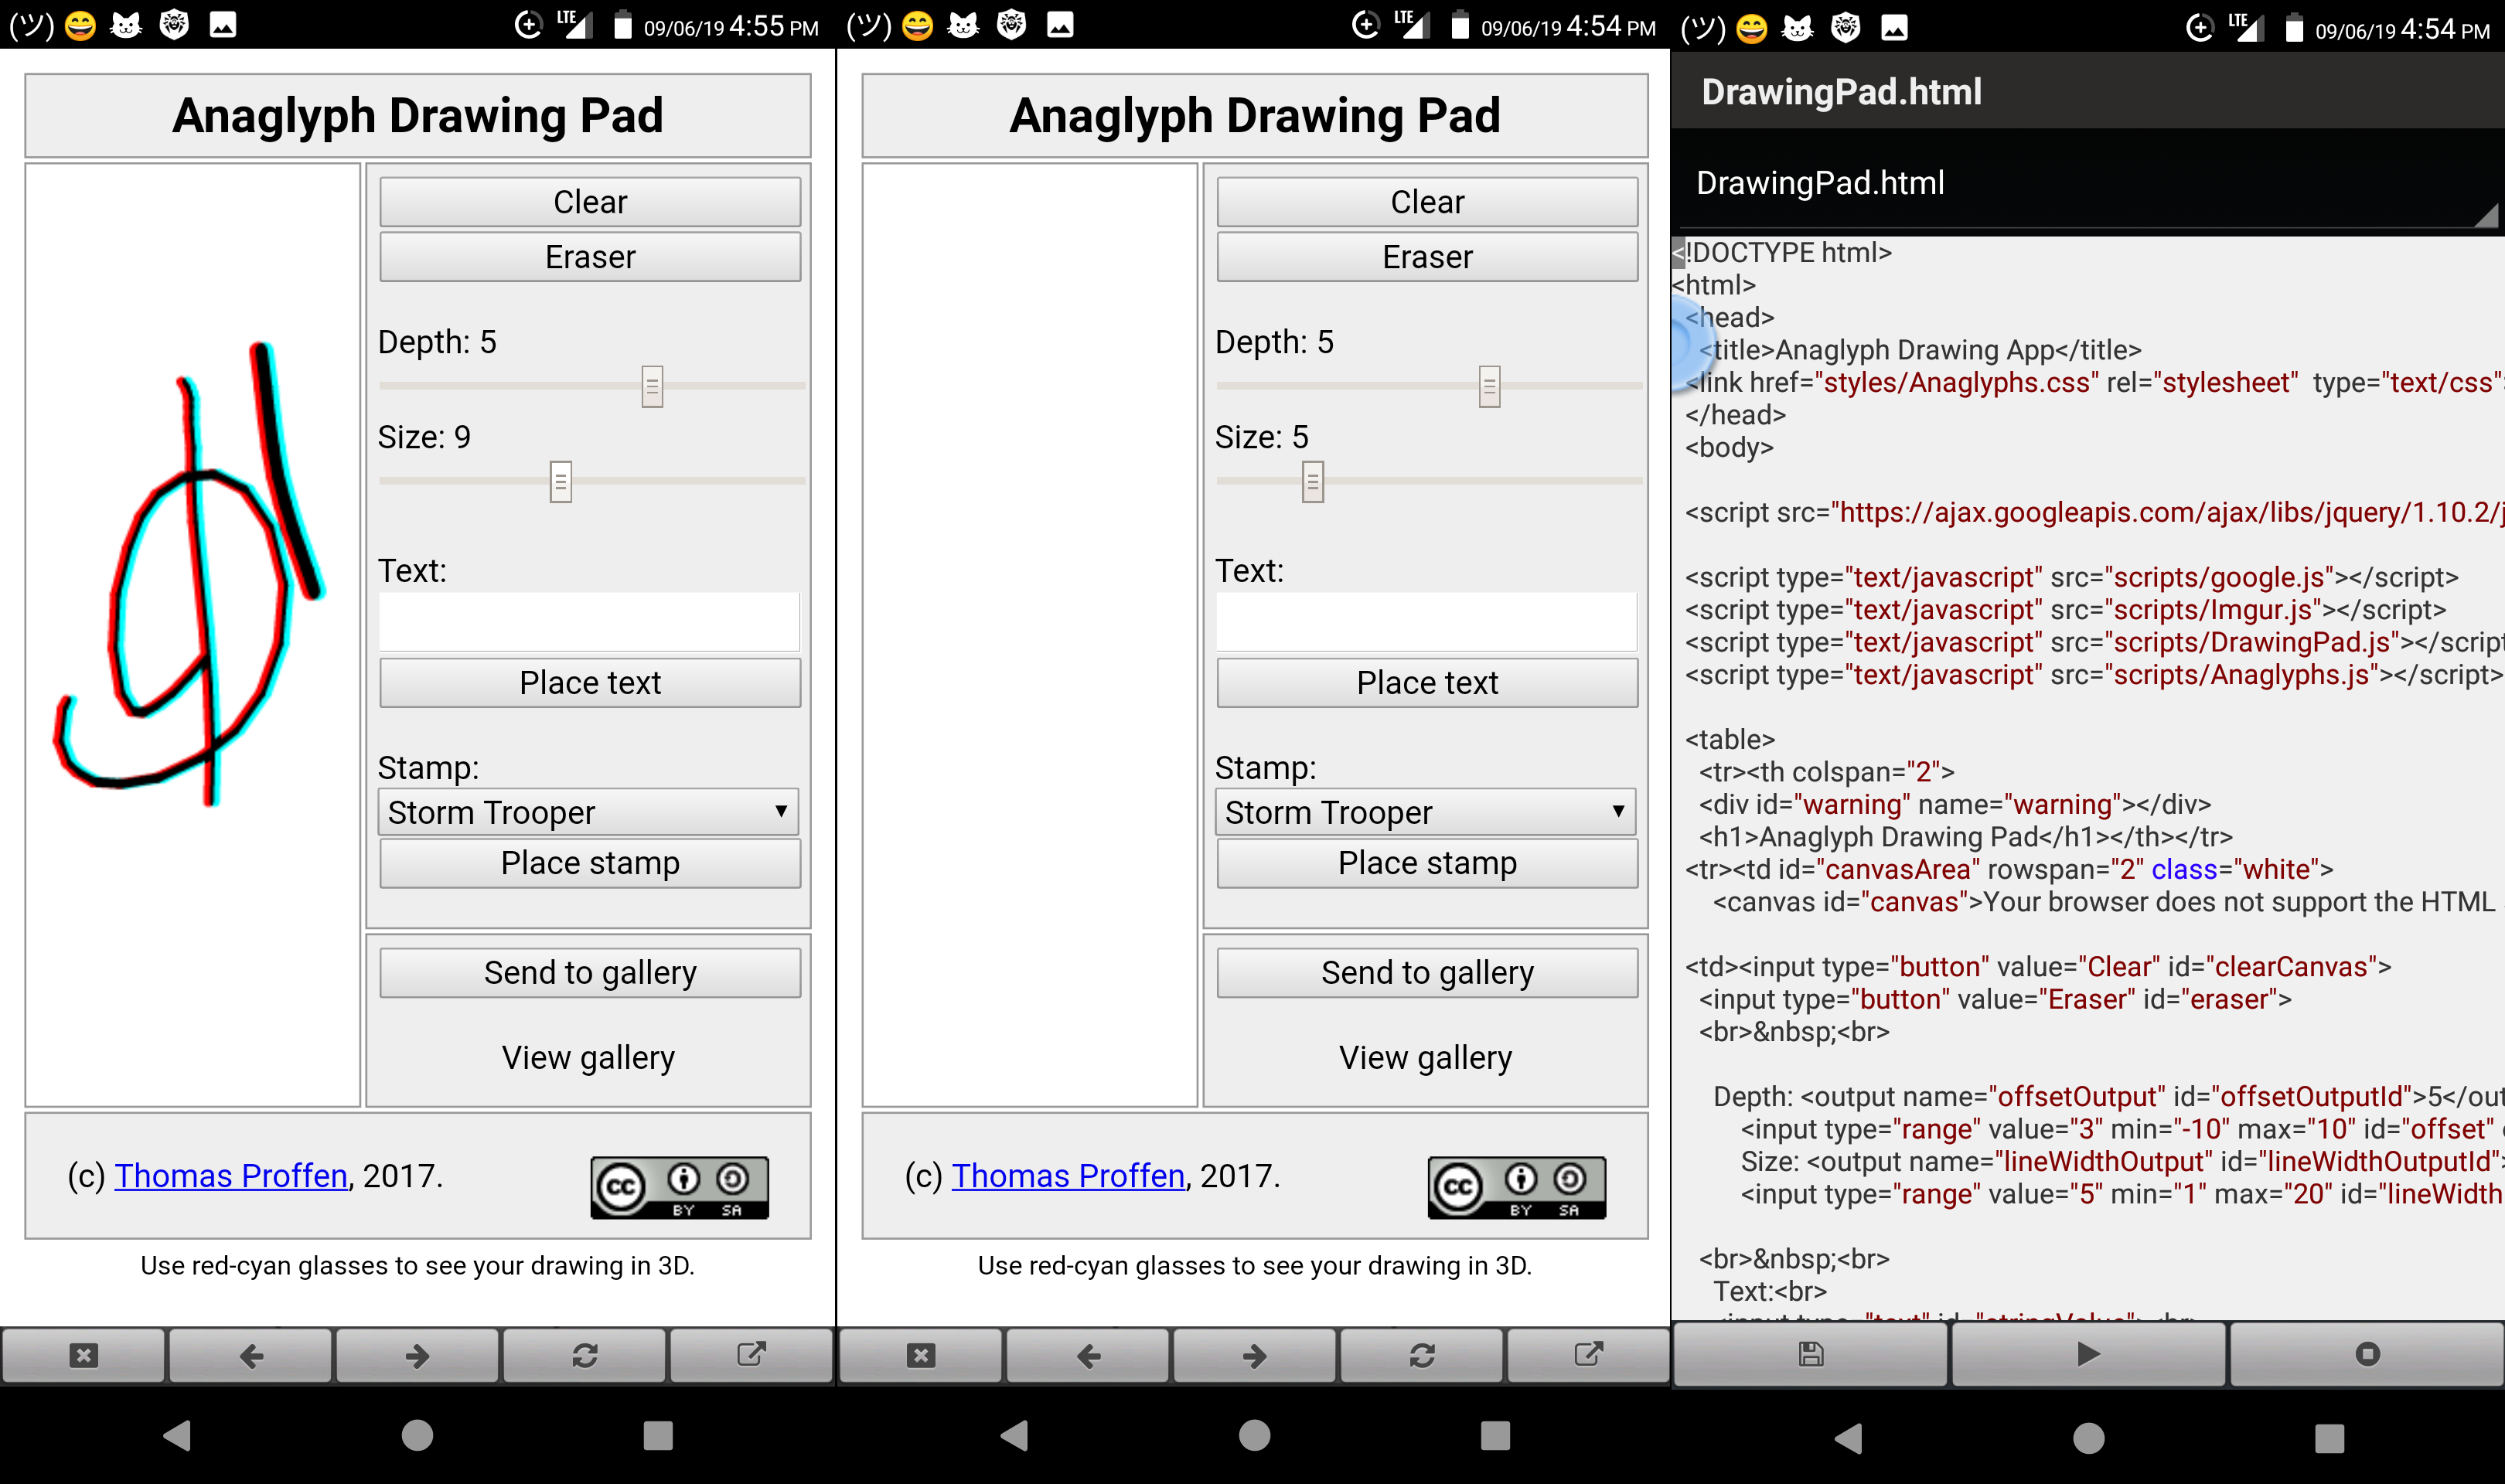
\includegraphics[width=\textwidth]{gfx/anaglyphweb_merged.png}

\vspace{.5cm}

\noindent\textbf{Bonus:} If possible, try to host the project as your own Github repository and make it accessible via Github pages. Please make sure to credit the original authors. Then, link the repository here: \url{https://hltdev8642.github.io/webgl-water/}

\end{document}
